\graphicspath{{./figures/pipeline/}}

\chapter{Data Pipeline}
We developed a pipeline (fig. \ref{fig:project_pipeline}) comprising (1) a data engineering pipeline, and (2) a data science pipeline.
We devoted significant part of our effort into following existing and developing best practices in data science development standards, so as to ensure reproducibility of results as well as reusability of methods and tools also in other use cases.
Among the key Python frameworks we used to attain that is was the McKinsey's Kedro \cite{kedro}.
The complete implementation is available in \cite{windstfgithub}.

\begin{figure}[H]
	\centering
    \caption{The project pipeline.}
    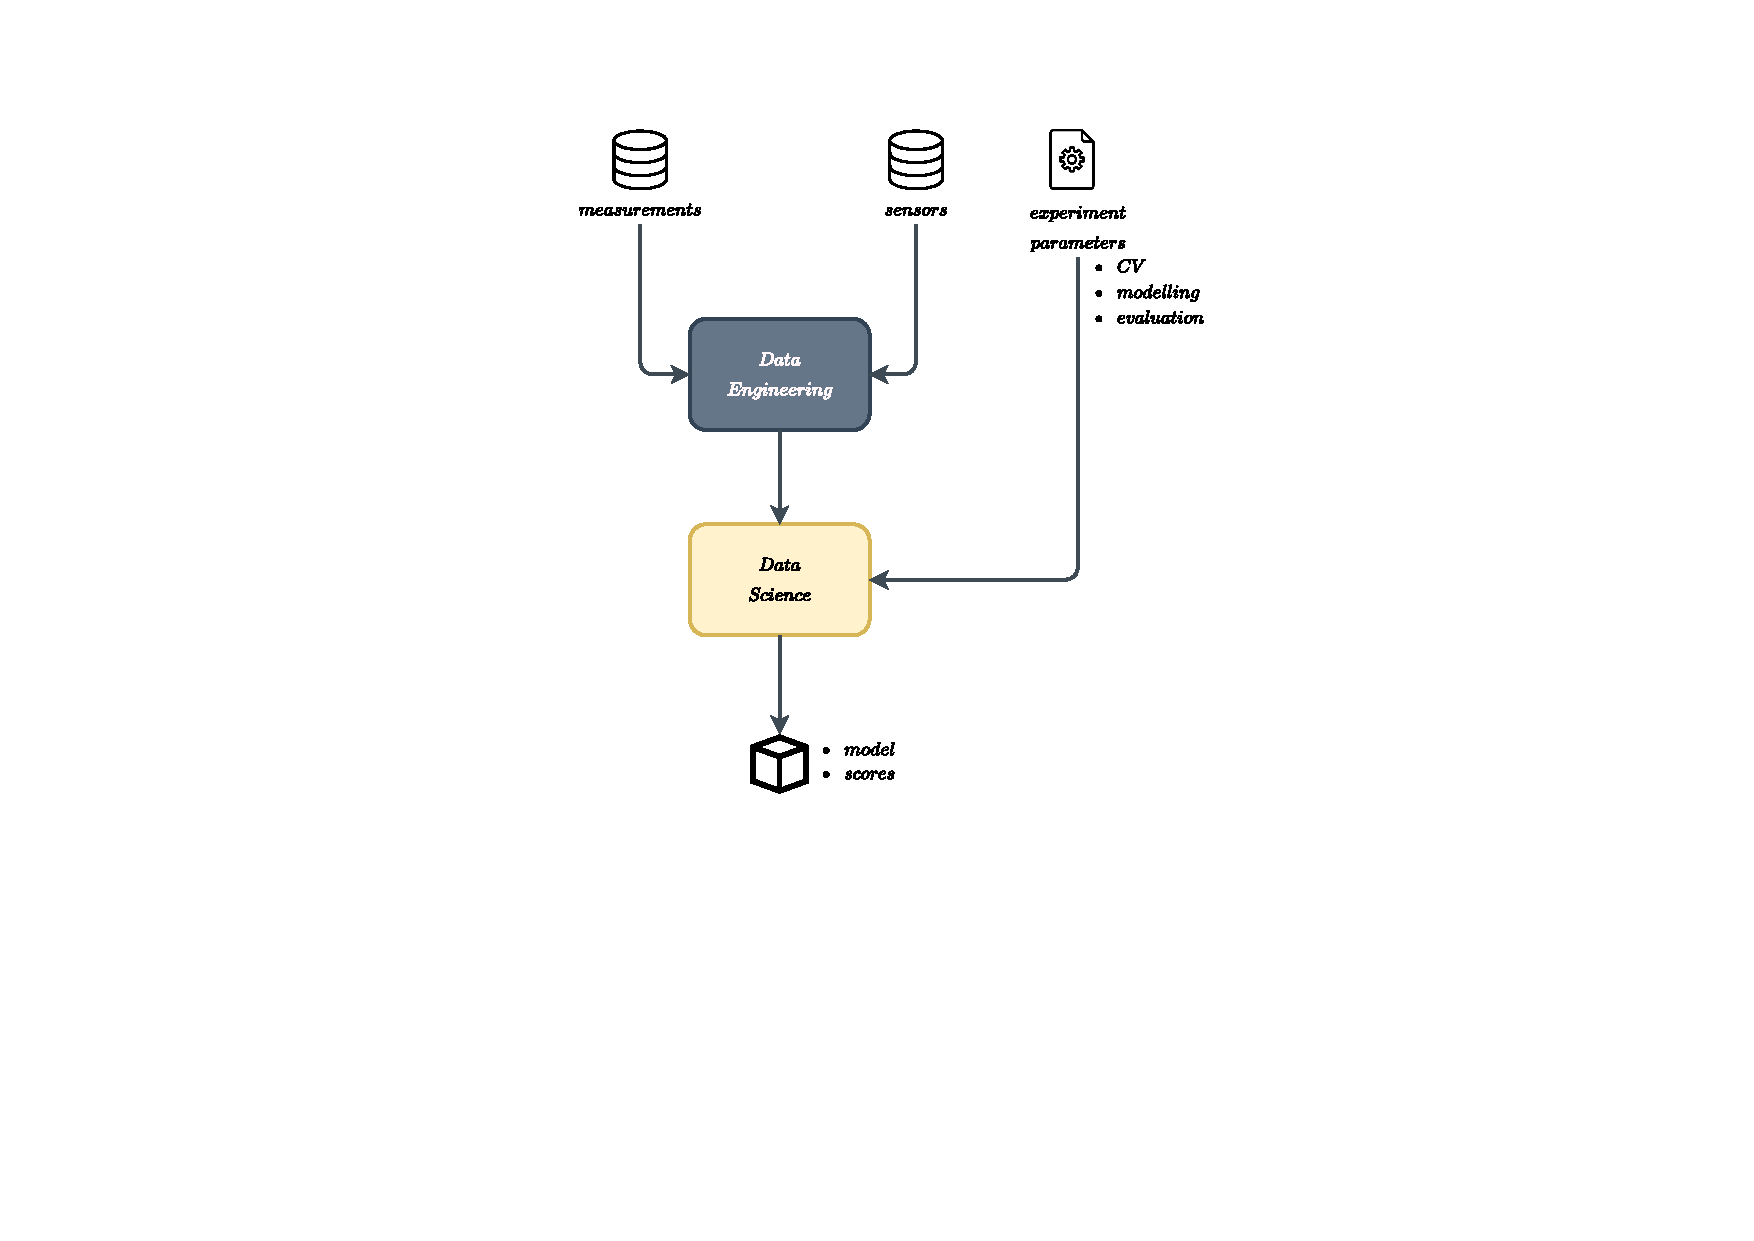
\includegraphics[width=0.8\linewidth,trim={7cm 7cm 7cm 2cm},clip]{pipeline_project.pdf}
    %\includesvg{pipeline_project}
	\label{fig:project_pipeline}
\end{figure}


\section{Data Engineering Pipeline}
The data engineering pipeline (fig. \ref{fig:pipeline_de}) encompasses all the data processing steps involved between (a) measurements and sensors datasets and (b) daily capacity factors, sensors graph inputs.

\begin{figure}[H]
	\centering
    \caption{The data engineering pipeline.}
    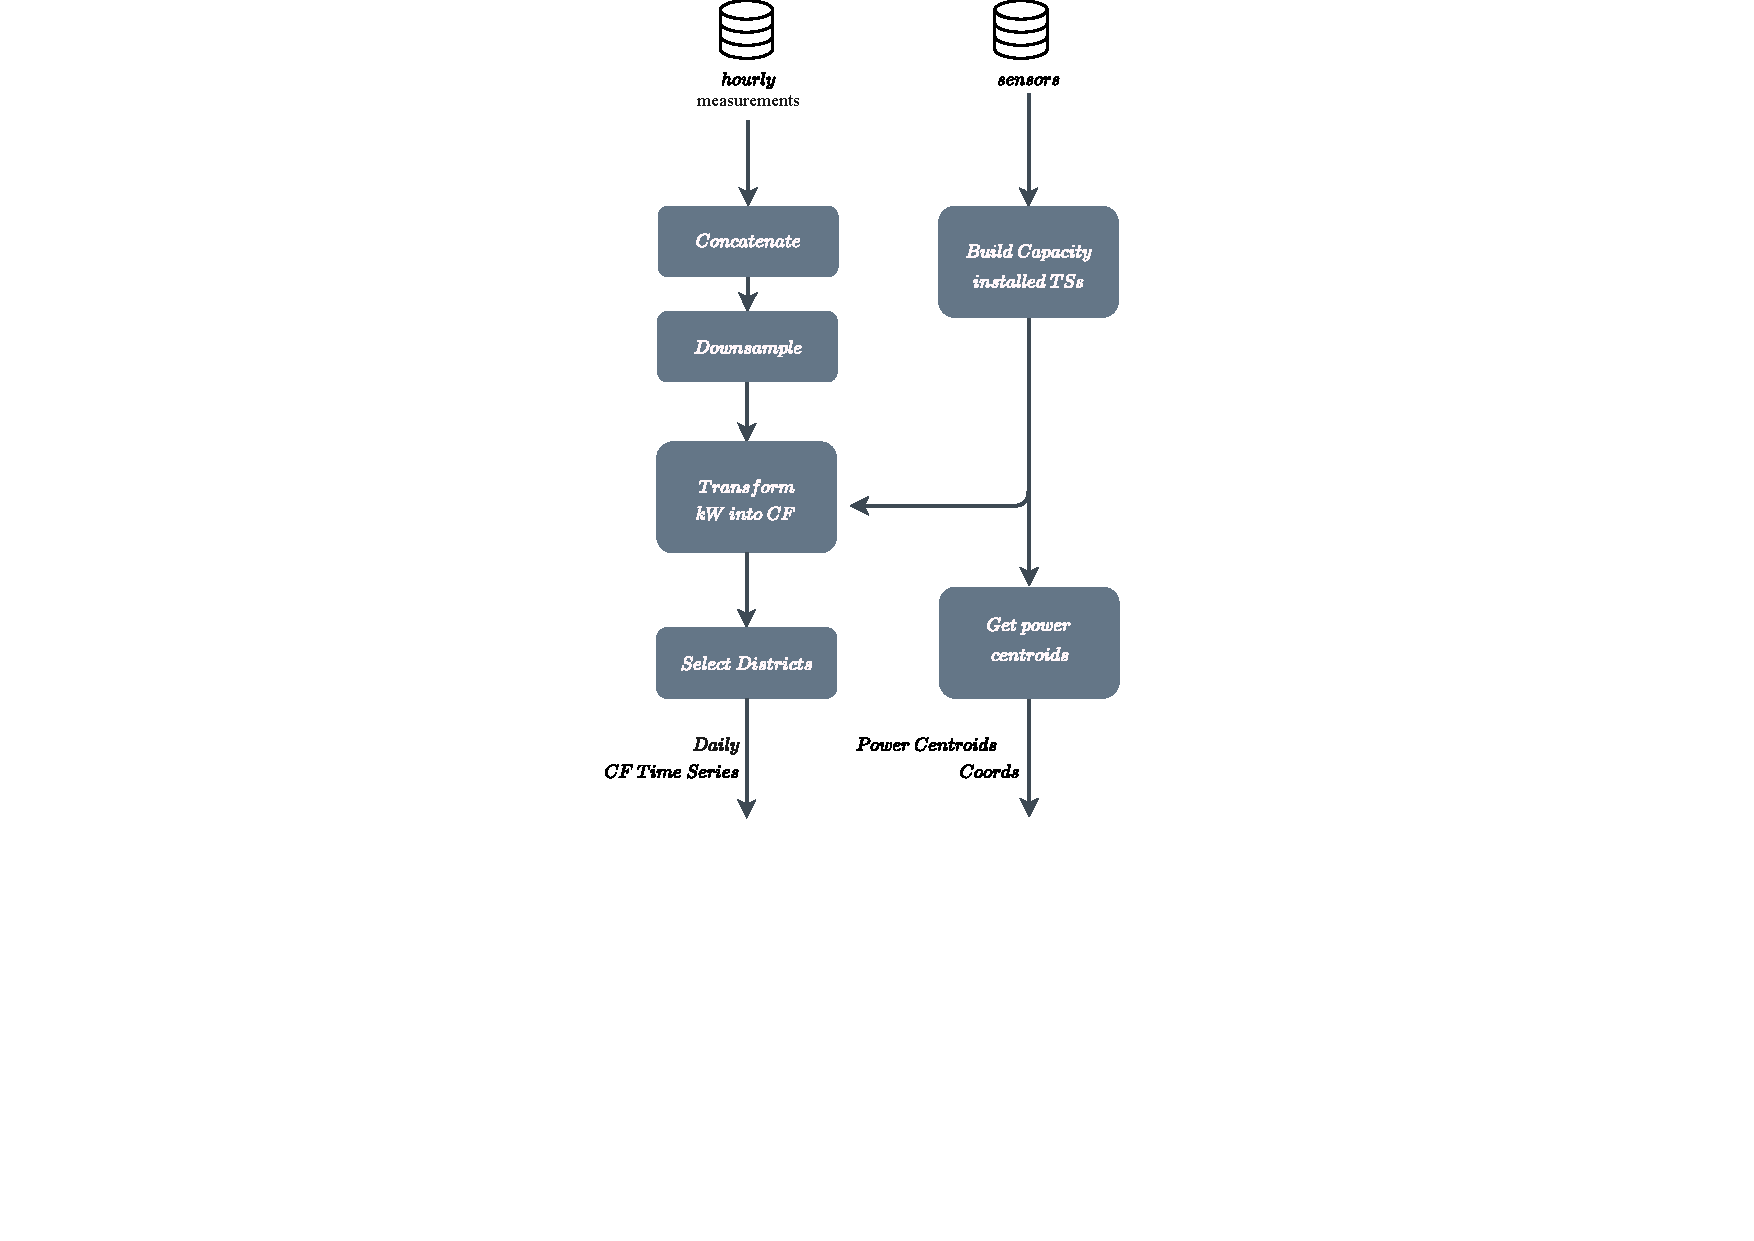
\includegraphics[width=1.0\linewidth,trim={7cm 7cm 7cm 0cm},clip]{pipeline_de.pdf}
	\label{fig:pipeline_de}
\end{figure}

\vspace{1em}
\noindent
\textbf{Get Capacity Installed Time Series.}  We load the sensors dataset and build a time series for the capacity installed in every district, essentially by grouping  turbine entries by district, and performing a cumulated sum of power ratings over the commissioning date-sorted entries.

\vspace{1em}
\noindent
\textbf{Get Power Centroids.}  A centroid position is defined for every district, not by its baricenter, but from the rated power-weighted average of all its single turbines coordinates. In practice, the power centroid changes its position every time  a new turbine is commissioned. We neglect this variation over time, and take the resulting average as sufficiently accurate for its purpose. Namely, we use the power centroids for calculating representative Euclidean distances between districts, which we used for the EDA and also when calculating the adjacency matrix initialization values for the graph-based spatio-temporal forecasting methods.

\vspace{1em}
\noindent
\textbf{Concatenate and Downsample.}  We concatenate the measurements dataset (power generated districtwise, in $kW$), which is provided for every year, into a single hourly dataframe, then downsample it into a daily measurements by summing same-day entries.

\vspace{1em}
\noindent
\textbf{Filter Districts.}   We filter out previously determined districts  which either represent outliers in spatial correlogram (3 from 296) or have zero installed capacity by 2015-01-01 (4 from 296).
Also, districts where in 2005-01-01 a single turbine represents more than 50\% of its installed capacity (18 districts in total).
Although the latter measure might represent a deviation from the industry use case, we perform it in favor of metrics representativity, as otherwise models overall performance metrics would be biased by low predictibility of ill-conditioned time series e.g. from districts where wind harvesting are still in early phases.
Finally we select the 33 districts in northern Germany with the highest capacity installed as of 2015-12-31.

\vspace{1em}
\noindent
\textbf{Transform kW to CF.}  Every entry in measurements time series dataset is normalized by the corresponding local installed capacity at the same day.
This results in daily time series for capacity factors in every district.

\pagebreak

\section{Data Science Pipeline}
The data science pipeline (fig. \ref{fig:pipeline_ds}) processes (a) user-defined parameters, (b) the capacity factors dataset resulting from the data engineering pipeline and, when required, also (c) the power centroids.

\begin{figure}[H]
	\centering
    \caption{The data engineering pipeline.}
    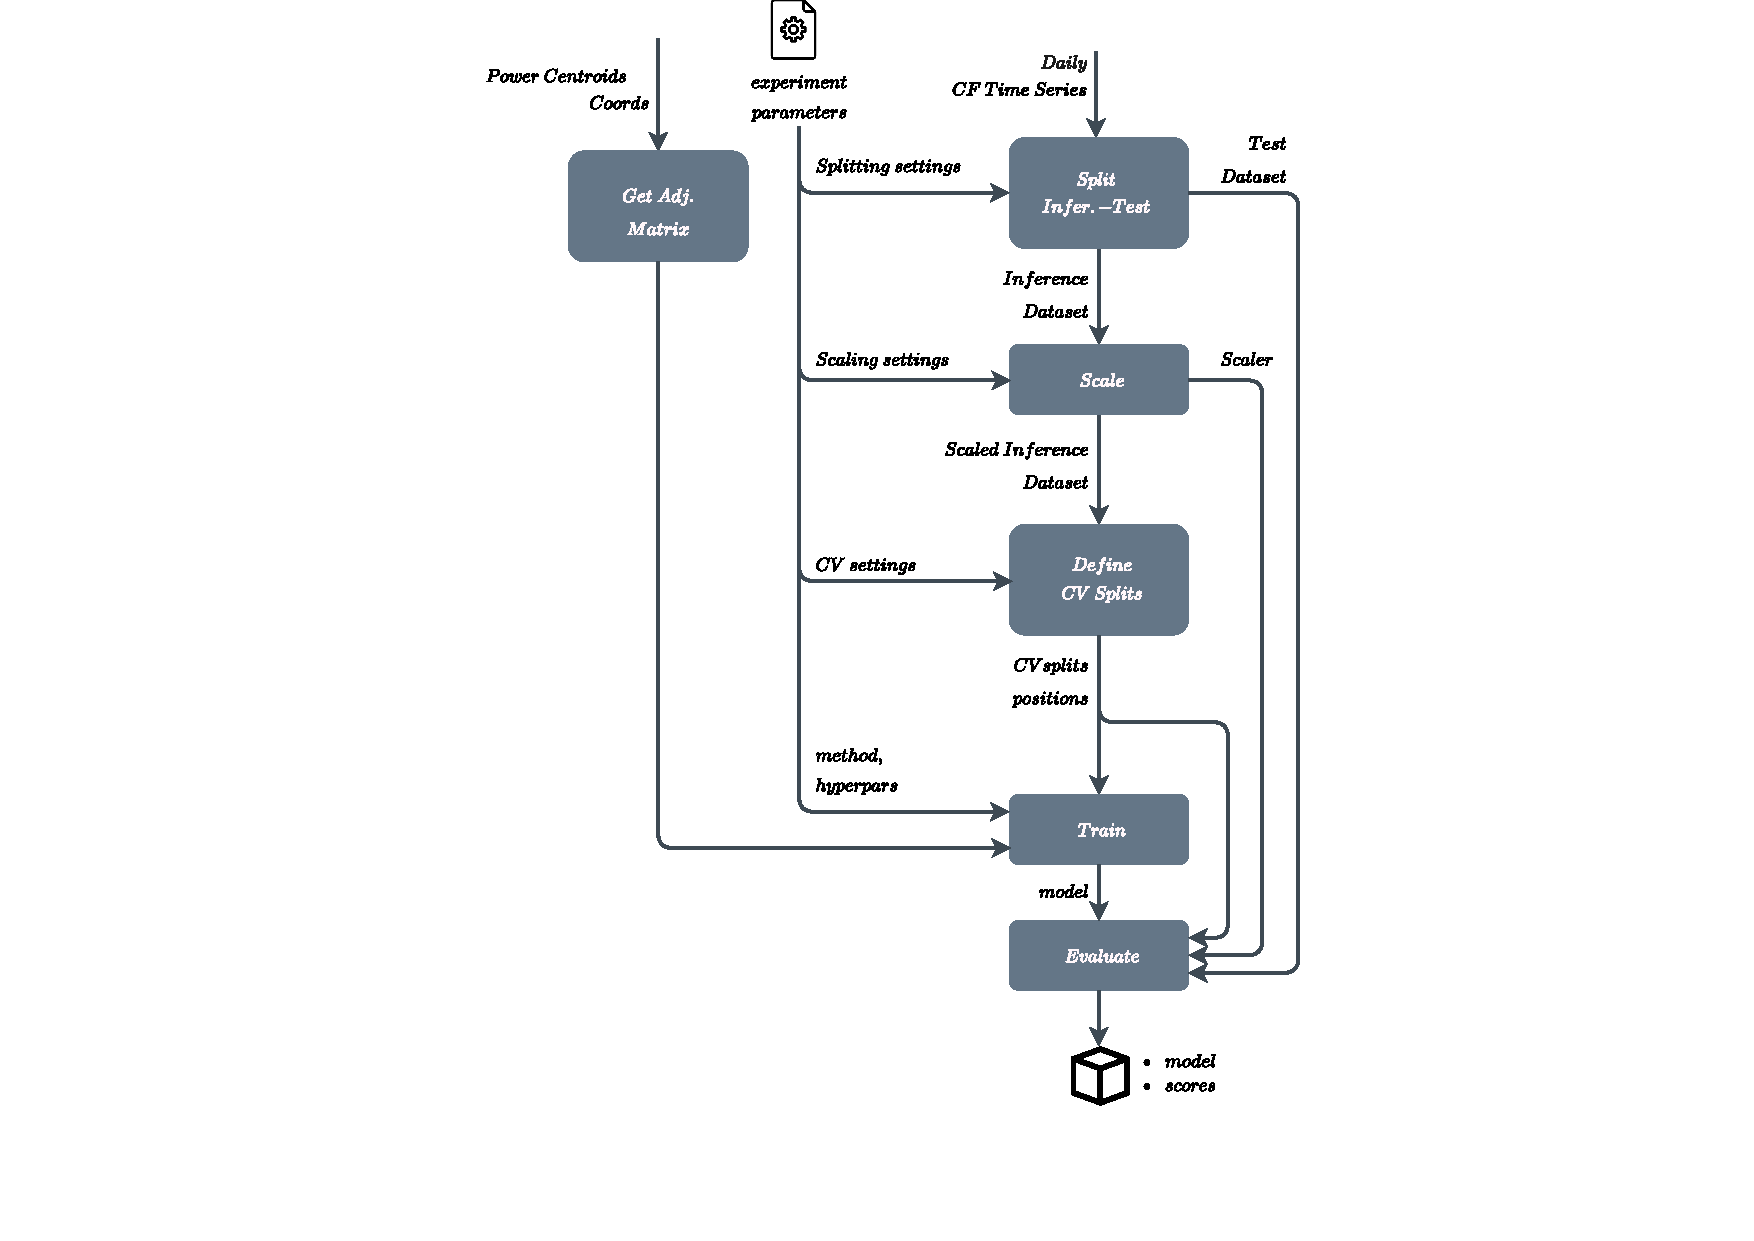
\includegraphics[width=1.0\linewidth,trim={6cm 2cm 6cm 0cm},clip]{pipeline_ds.pdf}
	\label{fig:pipeline_ds}
\end{figure}

\pagebreak

\vspace{1em}
\noindent
\textbf{Get Initial Adjacency Matrix.}  We calculate the matrix of the pairwise Euclidean distances and transform it into an adjacency matrix.
For initializing the values of the (constant) adjacency matrix in DCRNN or the self-adaptive adjacency matrix in the Graph WaveNet case, we follow the procedure in \cite{li2018dcrnn, wu2019graphwavenet} apply the Gaussian Kernel on the distances matrix, so that $A_{ij} = exp(-D_{ij}^2/2\sigma_{D}^2)$, where $\sigma_{D}$ is the standard deviation of the distances matrix.
Also as in \cite{li2018dcrnn}, we promote sparsity in the adjacency matrix for computational efficiency by thresholding the entries in the adjacency matrix.
However, instead of defining an arbitrary threshold value for $A_{ij}$, we prune adjacency values when the distances they are calculated from surpasses the decorrelation distance of 150 km.
We then normalize columnwise by the Frobenius Norm for faster convergence.
This node function is only processed in experiments for Graph Neural Network models, as they are the only methods considered which rely on an adjacency matrix.

\vspace{1em}
\noindent
\textbf{Define train-test split positions.} We follow the procedure described in section \ref{sec:reqs} for arbitrarily pick dates in 52 different weeks in 2015 to serve as the last train set and the one preceding the test set.
The positions are used to define 52 different train-test partitions, for which every model is trained and evaluated.

\vspace{1em}
\noindent
\textbf{Scale.}  We apply the user-defined sequence of scaling and offsetting methods on the inference data.

\vspace{1em}
\noindent
\textbf{Train.}  We train a model for every train-test split as well as one for the entire scaled model inference dataset.
In the case of single time series-modeling methods such as Holt-Winters Exponential Smoothing, the resulting model is actually a simple collection of univariate time series submodels.

\vspace{1em}
\noindent
\textbf{Evaluate.}  We make predictions using every trained model in the experiment, apply the inverse scaling (and offsetting) transformation and calculate overall model performance metrics averaged over train-test splits and over districts.